\chapter{Ornament catalog}

This document showcases two ornament libraries built on \texttt{pgfornament}:

\begin{itemize}
  \item \textbf{pgfhan} --- 78 Chinese traditional motifs (Chennan Zhang /
        LianTze Lim), catalogued in Part~I.
  \item \textbf{cantonese} --- original Cantonese decorative motifs
        (Lingnan, maritime, merchant), catalogued in Part~II.
\end{itemize}

\section{pgfhan usage}

\begin{verbatim}
\usepackage[object=pgfhan]{pgfornament}
\pgfornament[width=2cm, color=SeaGreen]{59}
\end{verbatim}

\begin{center}
  \pgfornament[width=2cm, color=SeaGreen]{59}
\end{center}

\section{Cantonese usage}

\begin{verbatim}
\usepackage[object=pgfhan]{pgfornament}
\usepackage{cantoneseornament}
\cantoneseornament[width=2cm, color=Maroon]{1}
\end{verbatim}

\begin{center}
  \cantoneseornament[width=2cm, color=Maroon]{1}
\end{center}

\section{Symmetry options}

Both families support \texttt{symmetry=h|v|c}:

\begin{center}
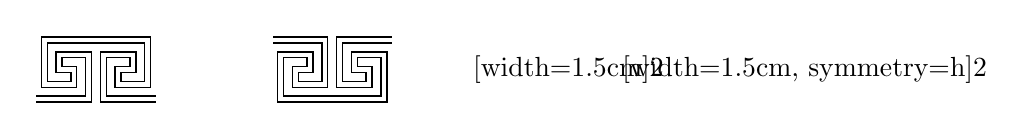
\begin{tikzpicture}
  \node at (0,0) {\pgfornament[width=1.5cm]{40}};
  \node at (3,0) {\pgfornament[width=1.5cm, symmetry=h]{40}};
  \node at (6,0) {\cantoneseornament[width=1.5cm]{2}};
  \node at (9,0) {\cantoneseornament[width=1.5cm, symmetry=h]{2}};
\end{tikzpicture}
\end{center}

\noindent
Left two: pgfhan~40. Right two: cantonese~2.

\tableofcontents
